\documentclass[crop,tikz]{standalone}

\input{../Presentation_MathsPreamble}

\usepackage[utf8]{inputenc}

% 'crop' is the default for v1.0, before it was 'preview'
%\usetikzlibrary{...}% tikz package already loaded by 'tikz' option

\begin{document}

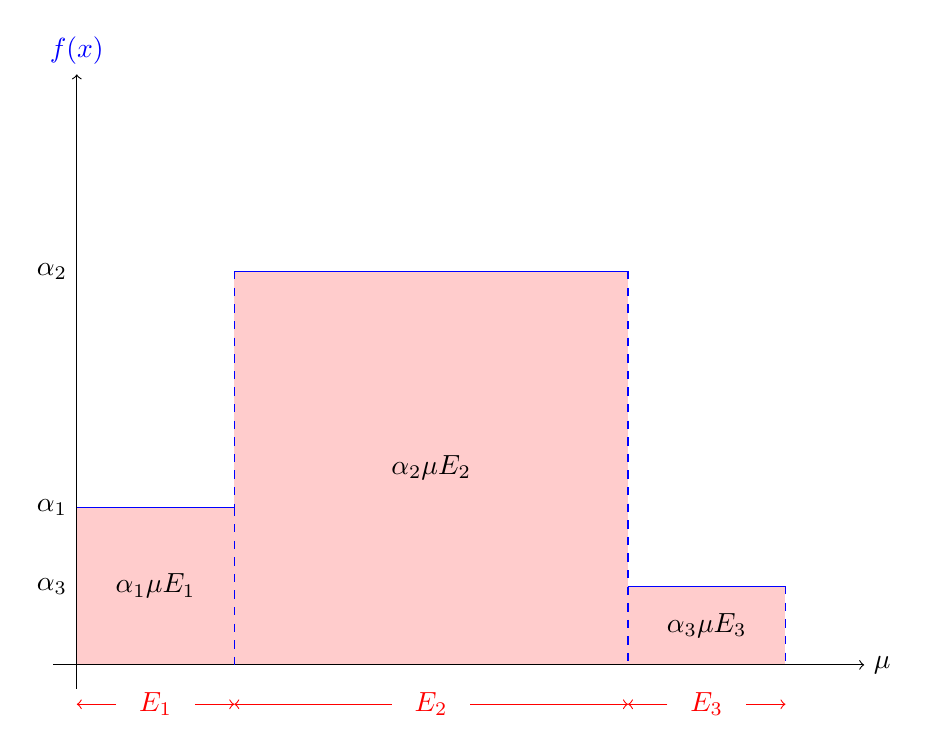
\begin{tikzpicture}

	%division of the range
	\draw[draw=none, fill=red!20!white] (0,0) rectangle (2,2);
	\node[align=center] at (1,1) {$\alpha_1\mu\bracs{E_1}$};
	\draw[draw=none, fill=red!20!white] (2,0) rectangle (7,5);
	\node[align=center] at (4.5,2.5) {$\alpha_2\mu\bracs{E_2}$};
	\draw[draw=none, fill=red!20!white] (7,0) rectangle (9,1);
	\node[align=center] at (8,0.5) {$\alpha_3\mu\bracs{E_3}$};

	\draw[->] (-0.3,0) -- (10,0) node[anchor=west] {$\mu$};
	\draw[->] (0,-0.3) -- (0,7.5);
	\node[anchor=south, color=blue] at (0,7.5) {$f(x)$};
	
	%simple function
	\draw[blue] (0,2) -- (2,2);
	\draw[blue, dashed] (2,2) -- (2,0);
	\node[anchor=east] at (0,2) {$\alpha_1$};
	\draw[blue] (2,5) -- (7,5);
	\draw[blue, dashed] (7,5) -- (7,0);
	\draw[blue, dashed] (2,5) -- (2,2);
	\node[anchor=east] at (0,5) {$\alpha_2$};
	\draw[blue] (7,1) -- (9,1);
	\draw[blue, dashed] (9,1) -- (9,0);
	\draw[blue, dashed] (7,5) -- (7,1);
	\node[anchor=east] at (0,1) {$\alpha_3$};
	
	%\mu-axis labels
	\draw[->, red] (1-0.5,-0.5) -- (0,-0.5); 
	\draw[->, red] (1+0.5,-0.5) -- (2,-0.5);
	\node[align=center, red] at (1,-0.5) {$E_1$};
	\draw[->, red] (4.5-0.5,-0.5) -- (2,-0.5); 
	\draw[->, red] (4.5+0.5,-0.5) -- (7,-0.5);
	\node[align=center, red] at (4.5,-0.5) {$E_2$};
	\draw[->, red] (8-0.5,-0.5) -- (7,-0.5); 
	\draw[->, red] (8+0.5,-0.5) -- (9,-0.5);
	\node[align=center, red] at (8,-0.5) {$E_3$};

\end{tikzpicture}

\end{document}